\documentclass[12pt]{article}
\usepackage{amsmath}
\usepackage{amssymb}
\usepackage{geometry}
\usepackage{enumerate}
\usepackage{natbib}
\usepackage{float}%稳定图片位置
\usepackage{graphicx}%画图
\usepackage[english]{babel}
\usepackage{a4wide}
\usepackage{indentfirst}%缩进
\usepackage{enumerate}%加序号
\usepackage{multirow}%合并行
\usepackage{graphicx}
\usepackage{enumerate}
\usepackage{booktabs}
\usepackage{geometry}
\usepackage{indentfirst}
\usepackage{mathrsfs}
\usepackage[T1]{fontenc}
\usepackage{mathtools}
\usepackage{amsthm}
\usepackage{babel}
\usepackage{listings}
\usepackage{subfigure}
\usepackage{caption}
\usepackage{pgfplots}
\usepackage{wrapfig}
\usepackage{rotating}
\usepackage[section]{placeins}
\usepackage{subfigure}
\usepackage{textcomp}
\usepackage[normalem]{ulem}
\usepackage{tabularx}
\usepackage{color}
\usepackage{mathrsfs}
\usepackage{setspace}
\usepackage[colorlinks,linkcolor=blue]{hyperref}%超链接
\title{\large UM-SJTU JOINT INSTITUTE\\PROBABILISTIC  METHODS IN
ENGINEERING\\(VE401)\\\ \\\ \\\ \\\ \\\ \\\ \\\ \\\
PROJECT 2 REPORT\\\ \\\ TEAM PROJECT GROUP 30 \\\ \\\ \\\ \\\ \\\ }
\author{Authors' Name and ID\\Chen Zhibo 515020910276\\Pan Chongdan 516370910121\\Shen Yuan 516370910122\\Xiang Zhiyuan 516370910126\\Zhan Yan 516370910206}
\date{Date: \today}

\begin{document}
\maketitle
\newpage
\tableofcontents
\newpage
\section{Synopsis}
The mass shooting problem in the United States is increasingly severe in recent years, and many statistic group has collected the relevant data for several years. Our group believe that the knowledge of statistical methods can be applied in the area of public security. So we based on the data obtained from Gun Violence Archive to analyze the distribution of numbers of occurrence of mass shooting in one day in the United States.
\par Following the example of the article $London$ $murders$: $a$ $predictable$ $pattern?$, at first we thought it may follow a Poisson distribution. However, the data shows from year 2013 to 2017, there is evidence to reject that the numbers of occurrence of mass shooting in one day follow a Poisson distribution, even if we test the data in each individual year, the hypotheses are all rejected.
\par But then, we find the most mass shooting occur on Saturday and Sunday, and we confirmed it depends on the weekdays.
\par Then we tested the hypotheses that the numbers of occurrence of mass shooting in one week follow a Poisson distribution, or the numbers of occurrence of mass shooting in one year follow a Poisson distribution. Unfortunately, there is evidence to reject these two hypotheses.
\par Then we narrowed down our test range, instead of testing the 5 years data at the same time, we just focused on the weekly data from January-June 2018. And at this time, we found there is no evidence the data does not follow a Poisson distribution with parameter $k=6.04$, that means the numbers of occurrence of mass shooting in one week may follow a Poisson distribution in a short period, like a single year.
\par Finally we got our conclusion, that is the occurrence of mass shootings depends on weekdays, and it is more likely to happen in weekends. And the numbers of occurrence of mass shooting in one week may follow a Poisson distribution in a short period, like a single year, but not in a long period, and the reason may be that the occurrence of mass shooting is not a random event. People may tend to shoot when the social security is not so good, it depends on many social factors, so in a short period, when the social and national conditions don't change a lot, the the numbers of occurrence of mass shooting in one week may follow a Poisson distribution, but in a long period, since the society and country are changing, which may cause the parameter $k$ of the Poisson distribution to change, so we can't simply use Poisson distribution to test the data in a long period.
\newpage
\section{Project Introduction}
The article $London$ $murders$: $a$ $predictable$ $pattern?$, written by David Spiegelhalter and Arthur Barnett [4], discusses the pattern of murders in London between April 2004 and September 2007 based on data of the London Metropolitan Police, obtained from the British Home Office. And in this project, we followed the example of David and Arthur, and instead of basing on the London murders, we focused on the social issue in the United States, that is Shooting Accident, especially the Mass Shooting problem. The mass shooting problem is increasingly severe in recent years, and our group believe that the knowledge of statistical methods can be applied in the area of public security. So we tried to base on the data obtained from Gun Violence Archive between January 2013 and December 2017 to analyze the mass shooting, hoping to find any pattern behind the data, so that we may be able to predict the occurrence of mass shooting in a period of time, and it may be helpful to prevent these issues to happen in the future.
\section{Exercise}
\subsection{Definitions of mass shooting and mass murder}
So, what is mass shooting? How we define it?
\par A mass shooting is  an incident involving multiple victims of firearms-related violence, and there is not a broadly accepted definition, for example, the United States'Congressional Research Service defines a "public mass shooting" as one in which four or more people selected indiscriminately, not including the perpetrator, are killed, and another unofficial definition of a mass shooting is an event involving the shooting(not necessarily resulting in death) of five or more people(sometimes four) with no "cooling-off period". And a mass murder is the act of murdering a number of people, typically simultaneously or over a relatively short period of time and in close geographic proximity, and FBI defines mass murder as murdering four or more persons during an event with no "cooling-off period" between murders.
\par Since there is not a broadly accepted definition of mass shooting, in our project, we decide to use the definition of Gun Violence Archive(GVA), and actually, if you comparing with other statistical data, you will find the GVA mass shooting numbers are higher than some other sources. Because GVA uses a purely statistical threshold to define mass shooting based ONLY on the numeric value of 4 or more shot or killed, not including the shooter. And GVA does not parse the definition to remove any subcategory of shooting, that means GVA does not exclude, set apart, caveat, or differentiate victims based upon the circumstances in which they were shot.
\subsection{Mass shooting data from 2013 to 2017}
\par To begin our project, first we collected numbers of mass shootings in one day from 2013 to 2017, and created a figure below. Based on the figure we found that the number of days with only one mass shooting happened is greatest, and then is the days with 2,3,4,5 mass shootings happened, and the number of days with 6 mass shootings happened is the smallest. Since in the article $London$ $murders$: $a$ $predictable$ $pattern?$, David Spiegelhalter and Arthur Barnett estimated that the London homicides follow a Poisson distribution with parameter $k=0.44$, and our figure showed there is a chance the mass shootings in the United States follow a Poisson distribution. But we needed to do some tests to confirm our hypothesis.
\begin{figure}[H]
\centering
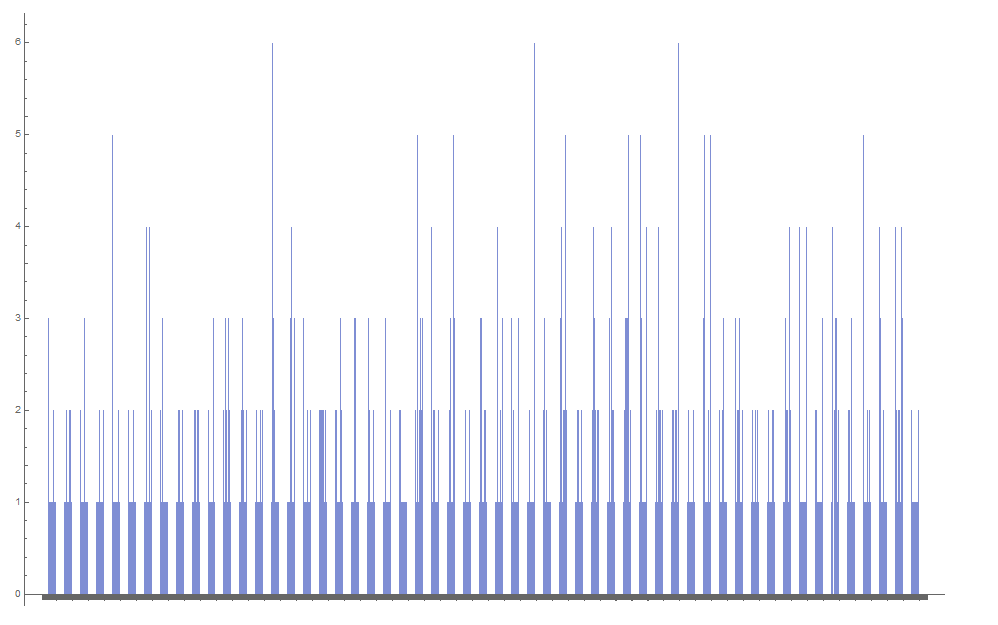
\includegraphics[scale=0.35]{Q2.jpg}
\caption{The data is from 2013 to 2017}
\end{figure}
\subsection{Test of Poisson distribution of mass shooting in US}
Here we decided to use Pearson's test to test our hypothesis, that is the mass shootings in the United States follow a Poisson distribution.
\par We use the data from GVA and get the number of mass shootings that happened in each day between January 1st, 2013 and December 31st, 2017:
\begin{table} [!htbp]
\begin{center}
\begin{tabular*} {14cm} {@{\extracolsep{\fill} }ccc}
\toprule
Numbers of mass shootings each day & numbers of days \\
\midrule
0 & 886 \\ \hline
1 & 540 \\ \hline
2 & 240 \\ \hline
3 & 102 \\ \hline
4 & 37  \\ \hline
5 & 15  \\ \hline
6 & 6   \\
\bottomrule
\end{tabular*}
\end{center}
\caption{Observed number of days with number of mass shootings from years 2013 to 2017}
\end{table}
\par The total mass shootings number is $540+240\times2+102\times3+37\times4+15\times5+6\times6=1585$. Now if the number of mass shootings follows poisson distribution, then the estimator for $k$ can be represent as below:
\begin{center}
$\hat k=\overline X=\dfrac{1585}{1826} \approx0.868$
\end{center}
\par Then we first calculate:
\begin{center}
$P[X=0]=\dfrac{e^{\hat k}\hat k^0}{0!} \approx0.41981$\\
$P[X=1]=\dfrac{e^{\hat k}\hat k^1}{1!} \approx0.36442$\\
$P[X=2]=\dfrac{e^{\hat k}\hat k^2}{2!} \approx0.15810$\\
$P[X=3]=\dfrac{e^{\hat k}\hat k^3}{3!} \approx0.04581$\\
$P[X=4]=\dfrac{e^{\hat k}\hat k^4}{4!} \approx0.00993$\\
$P[X=5]=\dfrac{e^{\hat k}\hat k^5}{5!} \approx0.00172$\\
$P[X\geq6]=1-P[X=0]-P[X=1]-P[X=2]-P[X=3]-P[X=4]-P[X=5]$\\
$=0.00025$
\end{center}
\par We can then replace the distribution of $X$ with that of a categorical random variable with parameters:
\begin{center}
$(p_0,p_1,p_2,p_3,p_5,p_6)=(0.41981,0.36442,0.15810,0.04581,0.00993,0.00172,0.00025)$
\end{center}
\par We then can calculate the expected frequencies $E_i=np_i$ with $n=1826$ as follows:
\begin{table} [!htbp]
\begin{center}
\begin{tabular*} {14cm} {@{\extracolsep{\fill} }ccc}
\toprule
Category i & Expected Frequency $E_i$ & Observed Frequency $Q_i$ \\
\midrule
0 & 766.57 & 886\\ \hline
1 & 665.43 & 540\\ \hline
2 & 288.69 & 240\\ \hline
3 & 83.65  & 102\\ \hline
4 & 18.13  &  37\\ \hline
5 & 3.14   &  15\\ \hline
6 & 0.4565 &  6 \\
\bottomrule
\end{tabular*}
\end{center}
\caption{Observed number of days and expected number of days with number of mass shootings from years 2013 to 2017}
\end{table}
\par However, if we cannot apply Pearson's test here, since our data doesn't satisfy the first criteria: $E[X_i]=np_i\geq1$ for all $i=1,...,k$.
\par The problem can be solved by combining the last two categories:
\begin{table} [!htbp]
\begin{center}
\begin{tabular*} {14cm} {@{\extracolsep{\fill} }ccc}
\toprule
Category i & Expected Frequency $E_i$ & Observed Frequency $Q_i$ \\
\midrule
0 & 766.57 & 886\\ \hline
1 & 665.43 & 540\\ \hline
2 & 288.69 & 240\\ \hline
3 & 83.65  & 102\\ \hline
4 & 18.13  &  37\\ \hline
5 & 3.60   &  21\\
\bottomrule
\end{tabular*}
\end{center}
\caption{Observed number of days and expected number of days with number of mass shootings from years 2013 to 2017}
\end{table}
Then let us test:
\begin{center}
$H_0$: The number of mass shootings happened in one day in United States follows a Poisson distribution with parameter $k=0.868$.
\end{center}
\par For $n=6$ categories, the statistic:
\begin{equation*}
X^2=\sum_{i=0}^{n-1}\dfrac{(O_i-E_i)^2}{E_i}
\end{equation*}
\par follows a chi-squared distribution with $n-1-m=4$ degrees of freedom. We testing the hypothesis at $\alpha=0.05$ and we will reject $H_0$ if $X^2\geq x_{0.05,4}=9.49$. Since we have:
\begin{center}
$X^2=\dfrac{(886-766.57)^2}{766.57}+\dfrac{(540-665.43)^2}{665.43}+\dfrac{(240-288.69)^2}{288.69}$\\
$+\dfrac{(102-83.65)^2}{83.65}+\dfrac{(37-18.13)^2}{18.13}+\dfrac{(21-3.60)^2}{3.60}\approx158.23$
\end{center}
\par Since $X^2\geq x_{0.05,4}$, we can reject $H_0$, which means there is no evidence that the number of mass shootings happened in one day in United States follows a Poisson distribution with parameter $k=0.868$.\\


\par Now, if we test the individual years for adherence to a Poisson distribution, what will we get?
\par First, we test the data for year 2013:
\begin{table} [!htbp]
\begin{center}
\begin{tabular*} {14cm} {@{\extracolsep{\fill} }ccc}
\toprule
Numbers of mass shooting each day & numbers of days \\
\midrule
0 & 198 \\ \hline
1 & 105 \\ \hline
2 & 47 \\ \hline
3 & 8 \\ \hline
4 & 6  \\ \hline
5 & 1  \\
\bottomrule
\end{tabular*}
\end{center}
\caption{Observed number of days with number of mass shootings in year 2013}
\end{table}
\par The total mass shootings number is $105+47\times2+8\times3+6\times4+1\times5=252$. Now if the number of mass shootings follows poisson distribution, then the estimator for $k$ can be represent as below:
\begin{center}
$\hat k=\overline X=\dfrac{252}{365} \approx0.6904$
\end{center}
\par Then we first calculate:
\begin{center}
$P[X=0]=\dfrac{e^{\hat k}\hat k^0}{0!} \approx0.50137$\\
$P[X=1]=\dfrac{e^{\hat k}\hat k^1}{1!} \approx0.34615$\\
$P[X=2]=\dfrac{e^{\hat k}\hat k^2}{2!} \approx0.11949$\\
$P[X=3]=\dfrac{e^{\hat k}\hat k^3}{3!} \approx0.02750$\\
$P[X=4]=\dfrac{e^{\hat k}\hat k^4}{4!} \approx0.00475$\\
$P[X\geq5]=1-P[X=0]-P[X=1]-P[X=2]-P[X=3]-P[X=4]$\\
$=0.00074$
\end{center}
\par We can then replace the distribution of $X$ with that of a categorical random variable with parameters:
\begin{center}
$(p_0,p_1,p_2,p_3,p_5)=(0.50137,0.34615,0.11949,0.02750,0.00475,0.00074)$
\end{center}
\par We then can calculate the expected frequencies $E_i=np_i$ with $n=365$ as follows:
\begin{table} [!htbp]
\begin{center}
\begin{tabular*} {14cm} {@{\extracolsep{\fill} }ccc}
\toprule
Category i & Expected Frequency $E_i$ & Observed Frequency $Q_i$ \\
\midrule
0 & 183.00 & 198\\ \hline
1 & 126.34 & 105\\ \hline
2 & 43.61 & 47\\ \hline
3 & 10.04  & 8\\ \hline
4 & 1.73  &  6\\ \hline
5 & 0.27   &  1\\
\bottomrule
\end{tabular*}
\end{center}
\caption{Observed number of days and expected number of days with number of mass shootings in year 2013}
\end{table}
\par However, if we cannot apply Pearson's test here, since our data doesn't satisfy the first criteria: $E[X_i]=np_i\geq1$ for all $i=1,...,k$.
\par The problem can be solved by combining the last two categories:
\begin{table} [!htbp]
\begin{center}
\begin{tabular*} {14cm} {@{\extracolsep{\fill} }ccc}
\toprule
Category i & Expected Frequency $E_i$ & Observed Frequency $Q_i$ \\
\midrule
0 & 183.00 & 198\\ \hline
1 & 126.34 & 105\\ \hline
2 & 43.61 & 47\\ \hline
3 & 10.04  & 8\\ \hline
4 & 2.00  &  7\\
\bottomrule
\end{tabular*}
\end{center}
\caption{Observed number of days and expected number of days with number of mass shootings in year 2013}
\end{table}
\par For $n=5$ categories, the statistic:
\begin{equation*}
X^2=\sum_{i=0}^{n-1}\dfrac{(O_i-E_i)^2}{E_i}
\end{equation*}
\par follows a chi-squared distribution with $n-1-m=3$ degrees of freedom.
\begin{center}
$X^2=\dfrac{(198-183.00)^2}{183.00}+\dfrac{(105-126.34)^2}{126.34}+\dfrac{(47-43.61)^2}{43.61}$\\
$+\dfrac{(8-10.04)^2}{10.04}+\dfrac{(7-2)^2}{2}\approx18.01$
\end{center}
\par So the P value of our test for year 2013 is 0.000438, it's quite small.\\


\par Then, let's test the data for year 2014:
\begin{table} [!htbp]
\begin{center}
\begin{tabular*} {14cm} {@{\extracolsep{\fill} }ccc}
\toprule
Numbers of mass shooting each day & numbers of days \\
\midrule
0 & 194 \\ \hline
1 & 103 \\ \hline
2 & 45 \\ \hline
3 & 18 \\ \hline
4 & 3  \\ \hline
5 & 1  \\ \hline
6 & 1  \\
\bottomrule
\end{tabular*}
\end{center}
\caption{Observed number of days with number of mass shootings in year 2014}
\end{table}
\par The total mass shootings number is $103+45\times2+18\times3+3\times4+1\times5+1\times6=270$. Now if the number of mass shootings follows poisson distribution, then the estimator for $k$ can be represent as below:
\begin{center}
$\hat k=\overline X=\dfrac{270}{365} \approx0.7397$
\end{center}
\par Then we first calculate:
\begin{center}
$P[X=0]=\dfrac{e^{\hat k}\hat k^0}{0!} \approx0.47724$\\
$P[X=1]=\dfrac{e^{\hat k}\hat k^1}{1!} \approx0.35303$\\
$P[X=2]=\dfrac{e^{\hat k}\hat k^2}{2!} \approx0.13057$\\
$P[X=3]=\dfrac{e^{\hat k}\hat k^3}{3!} \approx0.03220$\\
$P[X=4]=\dfrac{e^{\hat k}\hat k^4}{4!} \approx0.00595$\\
$P[X=5]=\dfrac{e^{\hat k}\hat k^5}{5!} \approx0.00088$\\
$P[X\geq6]=1-P[X=0]-P[X=1]-P[X=2]-P[X=3]-P[X=4]-P[X=5]$\\
$=0.00013$
\end{center}
\par We can then replace the distribution of $X$ with that of a categorical random variable with parameters:
\begin{center}
$(p_0,p_1,p_2,p_3,p_5,p_6)=(0.47724,0.35303,0.13057,0.03220,0.00595,0.00088,0.00013)$
\end{center}
\par We then can calculate the expected frequencies $E_i=np_i$ with $n=365$ as follows:
\begin{table} [H]
\begin{center}
\begin{tabular*} {14cm} {@{\extracolsep{\fill} }ccc}
\toprule
Category i & Expected Frequency $E_i$ & Observed Frequency $Q_i$ \\
\midrule
0 & 174.19 & 194\\ \hline
1 & 128.86 & 103\\ \hline
2 & 47.66 & 45\\ \hline
3 & 11.75  & 18\\ \hline
4 & 2.17 &  3\\ \hline
5 & 0.32 &  1\\ \hline
6 & 0.05  & 1\\
\bottomrule
\end{tabular*}
\end{center}
\caption{Observed number of days and expected number of days with number of mass shootings in year 2014}
\end{table}
\par However, if we cannot apply Pearson's test here, since our data doesn't satisfy the first criteria: $E[X_i]=np_i\geq1$ for all $i=1,...,k$.
\par The problem can be solved by combining the last three categories:
\begin{table} [!htbp]
\begin{center}
\begin{tabular*} {14cm} {@{\extracolsep{\fill} }ccc}
\toprule
Category i & Expected Frequency $E_i$ & Observed Frequency $Q_i$ \\
\midrule
0 & 174.19 & 194\\ \hline
1 & 128.86 & 103\\ \hline
2 & 47.66 & 45\\ \hline
3 & 11.75  & 18\\ \hline
4 & 2.54 &  5\\
\bottomrule
\end{tabular*}
\end{center}
\caption{Observed number of days and expected number of days with number of mass shootings in year 2014}
\end{table}
\par For $n=5$ categories, the statistic:
\begin{equation*}
X^2=\sum_{i=0}^{n-1}\dfrac{(O_i-E_i)^2}{E_i}
\end{equation*}
\par follows a chi-squared distribution with $n-1-m=3$ degrees of freedom.
\begin{center}
$X^2=\dfrac{(194-174.19)^2}{174.19}+\dfrac{(103-128.86)^2}{128.86}+\dfrac{(45-47.66)^2}{47.66}$\\
$+\dfrac{(18-11.75)^2}{11.75}+\dfrac{(5-2.54)^2}{2.54}\approx13.30$
\end{center}
\par The P value of our test for year 2014 is 0.004031, it's also quite small.\\


\par Then, let's test the data for year 2015:
\begin{table} [H]
\begin{center}
\begin{tabular*} {14cm} {@{\extracolsep{\fill} }ccc}
\toprule
Numbers of mass shooting each day & numbers of days \\
\midrule
0 & 164 \\ \hline
1 & 124 \\ \hline
2 & 42\\ \hline
3 & 21 \\ \hline
4 & 7  \\ \hline
5 & 6  \\ \hline
6 & 1  \\
\bottomrule
\end{tabular*}
\end{center}
\caption{Observed number of days with number of mass shootings in year 2015}
\end{table}
\par The total mass shootings number is $124+42\times2+21\times3+7\times4+6\times5+1\times6=335$. Now if the number of mass shootings follows poisson distribution, then the estimator for $k$ can be represent as below:
\begin{center}
$\hat k=\overline X=\dfrac{335}{365} \approx0.9178$
\end{center}
\par Then we first calculate:
\begin{center}
$P[X=0]=\dfrac{e^{\hat k}\hat k^0}{0!} \approx0.39939$\\
$P[X=1]=\dfrac{e^{\hat k}\hat k^1}{1!} \approx0.36657$\\
$P[X=2]=\dfrac{e^{\hat k}\hat k^2}{2!} \approx0.16822$\\
$P[X=3]=\dfrac{e^{\hat k}\hat k^3}{3!} \approx0.05146$\\
$P[X=4]=\dfrac{e^{\hat k}\hat k^4}{4!} \approx0.01181$\\
$P[X=5]=\dfrac{e^{\hat k}\hat k^5}{5!} \approx0.00217$\\
$P[X\geq6]=1-P[X=0]-P[X=1]-P[X=2]-P[X=3]-P[X=4]-P[X=5]$\\
$=0.00038$
\end{center}
\par We can then replace the distribution of $X$ with that of a categorical random variable with parameters:
\begin{center}
$(p_0,p_1,p_2,p_3,p_5,p_6)=(0.39939,0.36657,0.16822,0.05146,0.01181,0.00217,0.00038)$
\end{center}
\par We then can calculate the expected frequencies $E_i=np_i$ with $n=365$ as follows:
\begin{table}[H]
\begin{center}
\begin{tabular*} {14cm} {@{\extracolsep{\fill} }ccc}
\toprule
Category i & Expected Frequency $E_i$ & Observed Frequency $Q_i$ \\
\midrule
0 & 145.78 & 164\\ \hline
1 & 133.80 & 124\\ \hline
2 & 61.40 & 42\\ \hline
3 & 18.78 & 21\\ \hline
4 & 4.31 &  7\\ \hline
5 & 0.79 &  6\\ \hline
6 & 0.14  & 1\\
\bottomrule
\end{tabular*}
\end{center}
\caption{Observed number of days and expected number of days with number of mass shootings in year 2015}
\end{table}
\par However, if we cannot apply Pearson's test here, since our data doesn't satisfy the first criteria: $E[X_i]=np_i\geq1$ for all $i=1,...,k$.
\par The problem can be solved by combining the last three categories:
\begin{table} [!htbp]
\begin{center}
\begin{tabular*} {14cm} {@{\extracolsep{\fill} }ccc}
\toprule
Category i & Expected Frequency $E_i$ & Observed Frequency $Q_i$ \\
\midrule
0 & 145.78 & 164\\ \hline
1 & 133.80 & 124\\ \hline
2 & 61.40 & 42\\ \hline
3 & 18.78 & 21\\ \hline
4 & 5.24 &  14\\
\bottomrule
\end{tabular*}
\end{center}
\caption{Observed number of days and expected number of days with number of mass shootings in year 2015}
\end{table}
\par For $n=5$ categories, the statistic:
\begin{equation*}
X^2=\sum_{i=0}^{n-1}\dfrac{(O_i-E_i)^2}{E_i}
\end{equation*}
\par follows a chi-squared distribution with $n-1-m=3$ degrees of freedom.
\begin{center}
$X^2=\dfrac{(164-145.78)^2}{145.78}+\dfrac{(124-133.80)^2}{133.80}+\dfrac{(42-61.40)^2}{61.40}$\\
$+\dfrac{(21-18.78)^2}{18.78}+\dfrac{(14-5.24)^2}{5.24}\approx24.03$
\end{center}
\par The P value of our test for year 2015 is $2.46\times10^{-5}$, it's too small.\\


\par Then, let's test the data for year 2016:
\begin{table} [!htbp]
\begin{center}
\begin{tabular*} {14cm} {@{\extracolsep{\fill} }ccc}
\toprule
Numbers of mass shooting each day & numbers of days \\
\midrule
0 & 165 \\ \hline
1 & 98 \\ \hline
2 & 55\\ \hline
3 & 28 \\ \hline
4 & 12  \\ \hline
5 & 6  \\ \hline
6 & 2  \\
\bottomrule
\end{tabular*}
\end{center}
\caption{Observed number of days with number of mass shootings in year 2016}
\end{table}
\par The total mass shootings number is $98+55\times2+28\times3+12\times4+6\times5+2\times6=382$. Now if the number of mass shootings follows poisson distribution, then the estimator for $k$ can be represent as below:
\begin{center}
$\hat k=\overline X=\dfrac{382}{365} \approx1.047$
\end{center}
\par Then we first calculate:
\begin{center}
$P[X=0]=\dfrac{e^{\hat k}\hat k^0}{0!} \approx0.35114$\\
$P[X=1]=\dfrac{e^{\hat k}\hat k^1}{1!} \approx0.36749$\\
$P[X=2]=\dfrac{e^{\hat k}\hat k^2}{2!} \approx0.19230$\\
$P[X=3]=\dfrac{e^{\hat k}\hat k^3}{3!} \approx0.06709$\\
$P[X=4]=\dfrac{e^{\hat k}\hat k^4}{4!} \approx0.01755$\\
$P[X=5]=\dfrac{e^{\hat k}\hat k^5}{5!} \approx0.00367$\\
$P[X\geq6]=1-P[X=0]-P[X=1]-P[X=2]-P[X=3]-P[X=4]-P[X=5]$\\
$=0.00076$
\end{center}
\par We can then replace the distribution of $X$ with that of a categorical random variable with parameters:
\begin{center}
$(p_0,p_1,p_2,p_3,p_5,p_6)=(0.35114,0.36749,0.198230,0.06709,0.01755,0.00367,0.00076)$
\end{center}
\par We then can calculate the expected frequencies $E_i=np_i$ with $n=365$ as follows:
\begin{table} [!htbp]
\begin{center}
\begin{tabular*} {14cm} {@{\extracolsep{\fill} }ccc}
\toprule
Category i & Expected Frequency $E_i$ & Observed Frequency $Q_i$ \\
\midrule
0 & 128.17 & 165\\ \hline
1 & 134.13 & 98\\ \hline
2 & 70.19 & 55\\ \hline
3 & 24.49 & 28\\ \hline
4 & 6.41 &  12\\ \hline
5 & 1.34 &  6\\ \hline
6 & 0.28  & 2\\
\bottomrule
\end{tabular*}
\end{center}
\caption{Observed number of days and expected number of days with number of mass shootings in year 2016}
\end{table}
\par However, if we cannot apply Pearson's test here, since our data doesn't satisfy the first criteria: $E[X_i]=np_i\geq1$ for all $i=1,...,k$.
\par The problem can be solved by combining the last two categories:
\begin{table} [!htbp]
\begin{center}
\begin{tabular*} {14cm} {@{\extracolsep{\fill} }ccc}
\toprule
Category i & Expected Frequency $E_i$ & Observed Frequency $Q_i$ \\
\midrule
0 & 128.17 & 165\\ \hline
1 & 134.13 & 98\\ \hline
2 & 70.19 & 55\\ \hline
3 & 24.49 & 28\\ \hline
4 & 6.41 &  12\\ \hline
5 & 1.62 &  8\\
\bottomrule
\end{tabular*}
\end{center}
\caption{Observed number of days and expected number of days with number of mass shootings in year 2016}
\end{table}
\par For $n=6$ categories, the statistic:
\begin{equation*}
X^2=\sum_{i=0}^{n-1}\dfrac{(O_i-E_i)^2}{E_i}
\end{equation*}
\par follows a chi-squared distribution with $n-1-m=4$ degrees of freedom.
\begin{center}
$X^2=\dfrac{(165-128.17)^2}{128.17}+\dfrac{(98-134.13)^2}{134.13}+\dfrac{(55-70.19)^2}{70.19}$\\
$+\dfrac{(28-24.49)^2}{24.49}+\dfrac{(12-6.41)^2}{6.41}+\dfrac{(8-1.64)^2}{1.64}\approx53.65$
\end{center}
\par The P value of our test for year 2016 is $6.23\times 10^{-11}$. It's too small.\\


\par Then, let's test the data for year 2017:
\begin{table} [!htbp]
\begin{center}
\begin{tabular*} {14cm} {@{\extracolsep{\fill} }ccc}
\toprule
Numbers of mass shooting each day & numbers of days \\
\midrule
0 & 165 \\ \hline
1 & 110 \\ \hline
2 & 51\\ \hline
3 & 27 \\ \hline
4 & 9  \\ \hline
5 & 1  \\ \hline
6 & 2  \\
\bottomrule
\end{tabular*}
\end{center}
\caption{Observed number of days with number of mass shootings in year 2017}
\end{table}
\par The total mass shootings number is $110+51\times2+27\times3+9\times4+1\times5+2\times6=346$. Now if the number of mass shootings follows poisson distribution, then the estimator for $k$ can be represent as below:
\begin{center}
$\hat k=\overline X=\dfrac{346}{365} \approx0.9479$
\end{center}
\par Then we first calculate:
\begin{center}
$P[X=0]=\dfrac{e^{\hat k}\hat k^0}{0!} \approx0.38754$\\
$P[X=1]=\dfrac{e^{\hat k}\hat k^1}{1!} \approx0.36736$\\
$P[X=2]=\dfrac{e^{\hat k}\hat k^2}{2!} \approx0.17412$\\
$P[X=3]=\dfrac{e^{\hat k}\hat k^3}{3!} \approx0.05502$\\
$P[X=4]=\dfrac{e^{\hat k}\hat k^4}{4!} \approx0.01304$\\
$P[X=5]=\dfrac{e^{\hat k}\hat k^5}{5!} \approx0.00247$\\
$P[X\geq6]=1-P[X=0]-P[X=1]-P[X=2]-P[X=3]-P[X=4]-P[X=5]$\\
$=0.00045$
\end{center}
\par We can then replace the distribution of $X$ with that of a categorical random variable with parameters:
\begin{center}
$(p_0,p_1,p_2,p_3,p_5,p_6)=(0.38754,0.36736,0.17412,0.05502,0.01304,0.00247,0.00045)$
\end{center}
\par We then can calculate the expected frequencies $E_i=np_i$ with $n=365$ as follows:
\begin{table} [!htbp]
\begin{center}
\begin{tabular*} {14cm} {@{\extracolsep{\fill} }ccc}
\toprule
Category i & Expected Frequency $E_i$ & Observed Frequency $Q_i$ \\
\midrule
0 & 141.45 & 165\\ \hline
1 & 134.09 & 110\\ \hline
2 & 63.55 & 51\\ \hline
3 & 20.08 & 27\\ \hline
4 & 4.76 &  9\\ \hline
5 & 0.90 &  1\\ \hline
6 & 0.16  & 2\\
\bottomrule
\end{tabular*}
\end{center}
\caption{Observed number of days and expected number of days with number of mass shootings in year 2017}
\end{table}
\par However, we cannot apply Pearson's test here, since our data doesn't satisfy the first criteria: $E[X_i]=np_i\geq1$ for all $i=1,...,k$.
\par The problem can be solved by combining the last two categories:
\begin{table} [!htbp]
\begin{center}
\begin{tabular*} {14cm} {@{\extracolsep{\fill} }ccc}
\toprule
Category i & Expected Frequency $E_i$ & Observed Frequency $Q_i$ \\
\midrule
0 & 141.45 & 165\\ \hline
1 & 134.09 & 110\\ \hline
2 & 63.55 & 51\\ \hline
3 & 20.08 & 27\\ \hline
4 & 4.76 &  9\\ \hline
5 & 1.06 &  3\\
\bottomrule
\end{tabular*}
\end{center}
\caption{Observed number of days and expected number of days with number of mass shootings in year 2017}
\end{table}
\par For $n=6$ categories, the statistic:
\begin{equation*}
X^2=\sum_{i=0}^{n-1}\dfrac{(O_i-E_i)^2}{E_i}
\end{equation*}
\par follows a chi-squared distribution with $n-1-m=4$ degrees of freedom.
\begin{center}
$X^2=\dfrac{(165-141.45)^2}{141.45}+\dfrac{(110-134.09)^2}{134.09}+\dfrac{(51-63.55)^2}{63.55}$\\
$+\dfrac{(27-20.08)^2}{20.08}+\dfrac{(9-4.76)^2}{4.76}+\dfrac{(3-1.06)^2}{1.06}\approx20.44$
\end{center}
\par The P value of our test for year 2017 is 0.00041, it's quite small.\\


\par Since the P values of test for year 2013, 2014, 2015, 2016 and 2017 are 0.000438, 0.004031, $2.46\times10^{-5}$, $6.23\times 10^{-11}$ and 0.00041, so actually there is evidence that even for individual year, the numbers of mass shootings happened each day may not follows poisson distribution.
\par So, should we then change our direction of analysis, that means may be we should focus on the numbers of deaths or injuries caused by mass shootings in one day. However, after discussion, our group denied it. But from the data, we found the numbers of deaths or injuries caused by mass shootings in one day vary from 4 to 500! And according to the GVA's definition of mass shooting, this number cannot go down to 0,1,2,3. So obviously it's unreasonable to test the numbers of deaths or injuries caused by mass shootings. Also, through our common sense, the numbers of deaths or injuries depend on the circumstances of the crime scene.
\par But, should we draw a conclusion that the occurrence of mass shooting absolutely has nothing to do with the Poisson distribution? The answer is no.
\par Because we found the P value of individual year is much larger than the P value of years from 2013 to 2017. So we guessed that the numbers of mass shootings happened in one day follow a poisson distribution only in a short time period, like a month, or a week, that means the parameter $k$ of the poisson distribution may be different from year to year, month to month, or week to week, so for a longer time period, since the parameter $k$ of the poisson distribution is changing, it's impossible for us to determine a single parameter $k$ for a long period. To see this, we continued our analysis.
\newpage
\subsection{Distribution of mass shooting on weekdays and months}
This time, we analyzed the occurrence of a mass shooting on weekdays and months, and we got the figure below:\\ 
\begin{figure}[H]
\centering
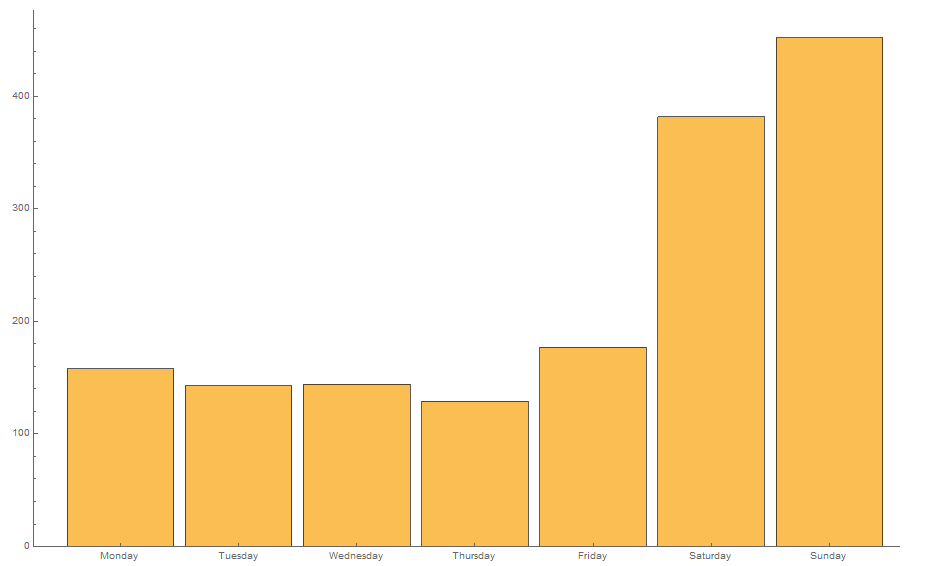
\includegraphics[scale=0.35]{Q4W.jpg}
\caption{Occurrence of a mass shooting on weekdays}
\end{figure}
It's obvious that most mass shooting occur on Saturday and Sunday, so it depends on the weekdays.
\begin{figure}[H]
\centering
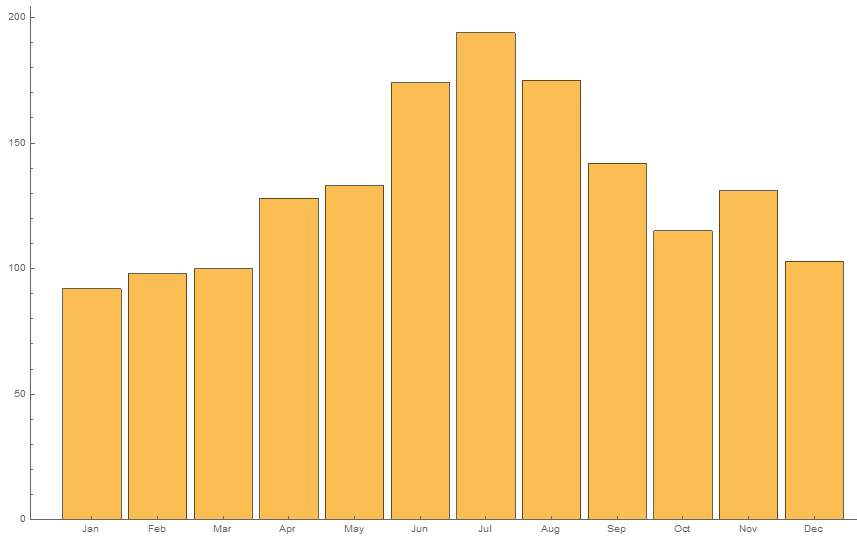
\includegraphics[scale=0.35]{Q4M.jpg}
\caption{Occurrence of a mass shooting on months}
\end{figure}
It's also obvious that more mass shooting occur in summer, so it also depends on the months.
\subsection{Analysis of mass shooting distribution on weekdays}
We were interested in this phenomenon, and we wanted to do some more precise calculation to prove the occurrence of a mass shooting does depend on the weekdays. And we wanted to figure out whether this phenomenon could be reason why we failed to accept that the mass shootings follow a Poisson distribution in the previous analysis.
\subsubsection{Whether Mass shootings follow Poisson Distribution}

\paragraph {Data does not Follow Poisson Distribution}

Using the software we  get the average number of shootings for each day in the week as shown below:

\begin{table} [!htbp]
\begin{center}
\begin{tabular*} {8 cm} {@{\extracolsep{\fill} }cc}
\toprule
Day & Average Number of Shooting\\
\midrule
Sunday	&	1.73 	\\ \hline
Monday	&	0.61	\\ \hline
Tuesday	&	0.55  \\ \hline
Wednesday&	0.55 	\\ \hline
Thursday	&	0.49 	\\ \hline
Friday 		&	0.68	\\ \hline
Saturday 	& 	1.46 	\\
\bottomrule
\end{tabular*}
\end{center}
\caption{Average Number of Shooting for Each Day }
\end{table}

We find that the average number of shootings on weekend is much larger than those on the weekdays. However, if it follows a Poisson distribution, it should be the same for weekend and weekdays. In the following part, we would use Fisher’s null hypothesis testing to reject the idea that it has same probability to have mass shootings on weekday and weekend. Because our data is so big, we can regard it as a normal distribution.


$$H_0:\mu_1=\mu_2$$

\begin{table} [!htbp]
\begin{center}
\begin{tabular*} {14cm} {@{\extracolsep{\fill} }cccc}
\toprule
Type & Data Number n &Average Number of Shooting $\overline X$ & Standard Deviation $S$\\
\midrule
Weekday	&	1304 & 0.58	& 0.8089\\ \hline
Weekend	&	522   &	1.60 & 1.3740\\ \hline
\bottomrule
\end{tabular*}
\end{center}
\caption{Average Number of Shooting for Weekday and Weekend}
\end{table}

As the variances have a big difference, we would use the pooled T-Test with unequal variances. Apply  Smith-Satterthwaite to get the $\gamma$.

$$\gamma=\frac{(S_1^2/n_1+S_2^2/n_2)^2}{\frac{(S_1/n_1)^2}{n_1-1}+\frac{(S_2/n_2)^2}{n_2-1}}=1247.7$$

we round it down to $\gamma=1247$,so

$$T_\gamma=\frac{(\overline X_1-\overline X_2)-(\mu_1-\mu_2)_0}{\sqrt{S_1^2/n_1+S_2^2/n_2}}=-8.805$$

From the table we get $t_{0.025,300}=1.968$ so we can see $T_\gamma >>t_{0.025,300}>t_{0.025,1247}$ so we can reject $H_0$ at the 0.05 level of significance.

By the Fisher’s null hypothesis testing, we can see the possibility for mass shootings in weekday and weekend is not same, so it would reject the idea that the number of shootings daily follows a Poisson distribution. Because if it follows a Poisson distribution, it would have same probabity to have mass shootings on weekday and weekend



\paragraph{Whether  Weekly Data Follow Poisson Distribution}

Now we had proved the occurrence of a mass shooting depends on weekdays, then it's no meaning for us to analyze the data daily. So the best way was to analyze the data weekly.
\par If we consider the data weekly, because the week starts on Sunday,we can get 260 full weeks form the date, we can get the results as below.

\begin{table} [!htbp]
\begin{center}
\begin{tabular*} {14cm} {@{\extracolsep{\fill} }ccc}
\toprule
Data Number n &Average Number of Shooting $\overline X$ & Standard Deviation $S$\\
\midrule
260 & 6.07	& 5.4448\\
\bottomrule
\end{tabular*}
\end{center}
\caption{Number of Shooting for Weeks}
\end{table}

To test if it follows Poisson Distribution, we would use Pearson’s chi-squared goodness-of-fit test. We rearrange our observed and expected number of mass shooting by combining into three adjacent categories.  We would use the Poisson distribution with k= 6.07.

$H_0$: the weekly number of mass shootings follows a Poisson distribution with the parameter $k=6.04$.

\begin{table} [!htbp]
\begin{center}
\begin{tabular*} {14cm} {@{\extracolsep{\fill} }ccc}
\toprule
Categorie &Actuall Number of Weeks& Expected Number of Weeks\\
\midrule
$[0,4)$ & 53	& 37.7\\ \hline
$[4,8)$ & 136	& 153.2\\ \hline
$[8,\infty)$ & 71	& 69.1\\
\bottomrule
\end{tabular*}
\end{center}
\caption{Categorie for Number of Shooting for Weeks}
\end{table}

Then we can get

$$X^2=\sum_{i=1}^{N}\frac{(O_i-E_i)^2}{E_i}=8.17$$


From the table we get $\chi^2_{0.05,1}=3.84$ so we can see $X^2>>\chi^2$ so we should  reject $H_0$ at the 0.05 level of significance.

If we only consider the individual year, we let 52 weeks to become a year and get the following results; (note: here the year is not same as the year we usually discussed)


\begin{table} [!htbp]
\begin{center}
\begin{tabular*} {14cm} {@{\extracolsep{\fill} }cccc}
\toprule
Year & Data Number n &Average Number of Shooting $\overline X$ & Standard Deviation $S$\\
\midrule
1	&	52 & 4.81	& 2.6645\\ \hline
2	&	52   &	5.19 & 2.6423\\ \hline
3	&	52 & 6.42	& 3.0828\\ \hline
4	&	52   &	7.27  & 3.7632\\ \hline
5	&	52 & 6.65	& 2.8414\\
\bottomrule
\end{tabular*}
\end{center}
\caption{Average Number of Shooting for  Week  by Year}
\end{table}



If we see it yearly, we would find the standard deviation in each individual year is much smaller than we consider it as a whole. Here we would test the first year as an example to see whether it following a Poisson distribution in each individual year.


$H_0$: the weekly number of mass shootings follows a Poisson distribution with the parameter $k=4.81$.


\begin{table} [!htbp]
\begin{center}
\begin{tabular*} {14cm} {@{\extracolsep{\fill} }ccc}
\toprule
Categorie &Actuall Number of Weeks& Expected Number of Weeks\\
\midrule
$[0,4)$ & 16	& 15.2\\ \hline
$[4,8)$ & 29	& 30.8\\ \hline
$[8,\infty)$ & 7	& 6.0\\
\bottomrule
\end{tabular*}
\end{center}
\caption{Categorie for Number of Shooting for First 52 Weeks}
\end{table}

Then we can get

$$X^2_1=\sum_{i=1}^{N}\frac{(O_i-E_i)^2}{E_i}=0.33$$


From the table we get $\chi^2_{0.05,1}=3.84$ so we can see $X^2_1<\chi^2$ so we should  not reject $H_0$ at the 0.05 level of significance.

Similarly, we can also not reject the idea the number of mass shootings for week follows a Poisson distribution in each individual year except for fourth 52 Weeks which is 2016.


\begin{table} [!htbp]
\begin{center}
\begin{tabular*} {14cm} {@{\extracolsep{\fill} }ccc}
\toprule
Categorie &Actuall Number of Weeks& Expected Number of Weeks\\
\midrule
$[0,4)$ & 14	& 12.5\\ \hline
$[4,8)$ & 29	& 31.5\\ \hline
$[8,\infty)$ & 9	& 8.0\\
\bottomrule
\end{tabular*}
\end{center}
\caption{Categorie for Number of Shooting for Second 52 Weeks}
\end{table}



\begin{table} [!htbp]
\begin{center}
\begin{tabular*} {14cm} {@{\extracolsep{\fill} }ccc}
\toprule
Categorie &Actuall Number of Weeks& Expected Number of Weeks\\
\midrule
$[0,4)$ & 6	& 6.1\\ \hline
$[4,8)$ & 31	& 29.5\\ \hline
$[8,\infty)$ & 15	& 16.4\\
\bottomrule
\end{tabular*}
\end{center}
\caption{Categorie for Number of Shooting for Third 52 Weeks}
\end{table}




\begin{table} [!htbp]
\begin{center}
\begin{tabular*} {14cm} {@{\extracolsep{\fill} }ccc}
\toprule
Categorie &Actuall Number of Weeks& Expected Number of Weeks\\
\midrule
$[0,4)$ & 9	& 3.6\\ \hline
$[4,8)$ & 23	& 25.5\\ \hline
$[8,\infty)$ & 20	& 22.9\\
\bottomrule
\end{tabular*}
\end{center}
\caption{Categorie for Number of Shooting for Fourth 52 Weeks}
\end{table}




\begin{table} [!htbp]
\begin{center}
\begin{tabular*} {14cm} {@{\extracolsep{\fill} }ccc}
\toprule
Categorie &Actuall Number of Weeks& Expected Number of Weeks\\
\midrule
$[0,4)$ & 8	& 5.3\\ \hline
$[4,8)$ & 24	& 28.5\\ \hline
$[8,\infty)$ & 20	& 18.2\\
\bottomrule
\end{tabular*}
\end{center}
\caption{Categorie for Number of Shooting for Fifth 52 Weeks}
\end{table}

Then we can get
$$X^2_2=\sum_{i=1}^{N}\frac{(O_i-E_i)^2}{E_i}=0.52$$
$$X^2_3=\sum_{i=1}^{N}\frac{(O_i-E_i)^2}{E_i}=0.20$$
$$X^2_4=\sum_{i=1}^{N}\frac{(O_i-E_i)^2}{E_i}=8.85$$
$$X^2_5=\sum_{i=1}^{N}\frac{(O_i-E_i)^2}{E_i}=2.28$$



To conclude, we would say the number of mass shootings for weeks on a large time scale does not follow a Poisson distribution. But for a  relative small time period, like one year, the number appear to follow the poisson distribution

It may because the k for the Poisson distribution is always changing, it may be affected by the economic or social security, it needs further analysis to give a more concrete result. But for a short time, the k for Poisson is relative stable.

\subsection{Weeks with n Shootings}


\subsubsection{Predicted and Actual Number of Weeks with n Shootings}

By the data above we can draw the actual graph like below.

\begin{figure}[H]
\begin{center}
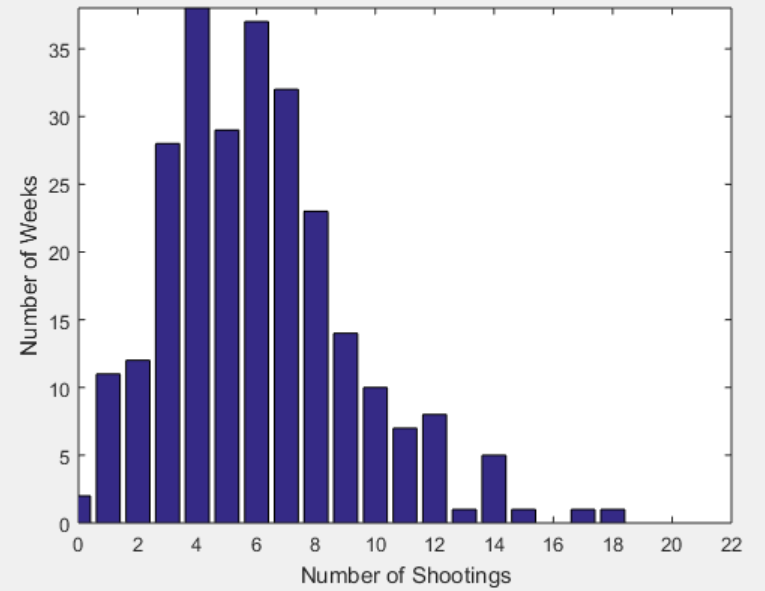
\includegraphics[width=10cm]{actual.png}
\caption{Actual Number of Weeks with n Shootings}
\end{center}
\end{figure}

Since we believe the number for mass shooting for long time period does not follow the Poisson distribution, here we would calculate the five years separately then add it together, and we get the following graph for the predicted number.


\begin{figure}[H]
\begin{center}
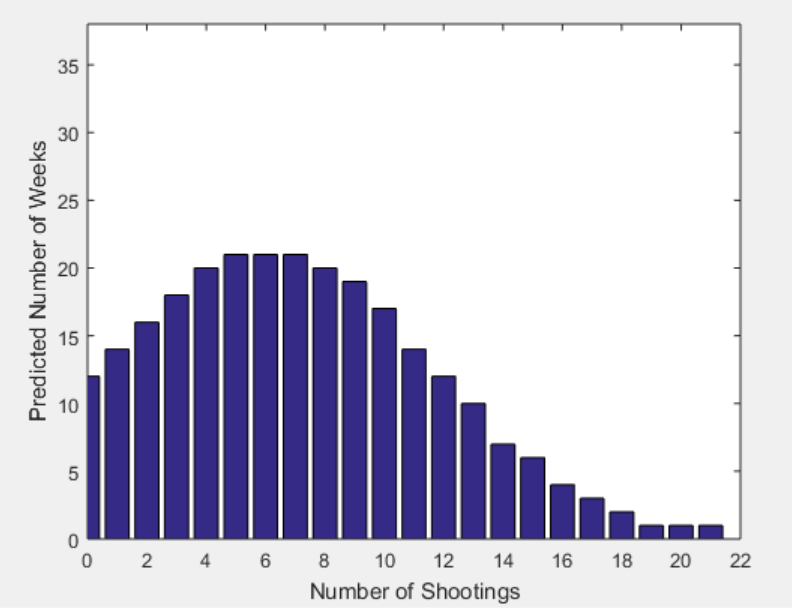
\includegraphics[width=10cm]{Predicted.png}
\caption{Predicted Number of Weeks with n Shootings with Poisson Distribution}
\end{center}
\end{figure}
\subsection{Study of confidence interval for $k$}
 Based on the method of maximum likelihood, we use $\bar X \ $to serve as the estimator $\hat {k}$ for $k$, which is proved in the lecture slide. As one essential assumption for a Poisson distribution is that ``the number of `arrivals' during non-overlapping time intervals are independent'', we can know that
\begin{equation*}
E[\bar X]=k, Var \bar X=k/n.
\end{equation*}
\par In our case, the sample size is large enough for us to reasonably assume that $\bar X$ follows a normal distribution with $E[\bar X]=k, Var \bar X=k/n$. Accordingly, the statistic $Z=\frac{\bar X-k}{\sqrt{k/n}}$ follows a standard normal distribution. It follows that a $100(1-\alpha)\%$ confidence interval for k is
\begin{equation*}
\bar X \pm z_{\alpha/2} \sqrt{k/n}
\end{equation*}
which is identical to the form that
\begin{equation*}
\hat k \pm z_{\alpha/2} \sqrt{k/n}
\end{equation*}
\par Nevertheless, the confidence interval depends on the parameter $k$ we hope to estimate. We can solve this problem by replacing $k$ by $\hat k$ and the interval becomes
\begin{equation*}
\hat k \pm z_{\alpha/2} \sqrt{\hat k/n}
\end{equation*}
In this way, we actually replace $\sigma $ by $S$, so we need to change $z_{\alpha/2}$ to $t_{\alpha/2}$. Notwithstanding, considering that our sample size is large enough for the central limit theorem to hold, it is rational for us to neglect the very subtle difference between $z_{\alpha/2}$ and $t_{\alpha/2}$ so that our solution can be simplified.
\par Using the weekly data of the years 2013 to 2017, we have can know that there are 262 weeks and the total number of mass shootings is 1585. Thus, we have:
\begin{equation*}
\hat k \pm z_{\alpha/2} \sqrt{\hat k/n}=[ 5.75,6.35 ].
\end{equation*}
\par \qed\
\subsection{Study of weekly data of Jan-Jun 2018 for Poisson distribution}
Using the weekly data of January to June 2018, we can know that there are 26 weeks and the total number of mass shootings is 157 in that period. Hence, the estimate for $k$ is $\hat{k}_{2018}=\bar X=157/26=6.04$, which falls into the confidence interval calculated above. The data are shown in the following table:
\begin{center}
\begin{tabular}{|c|c|c|c|c|c|c|c|c|c|c|c|c|c|c|c|c|c|}
\hline
\# Mass Shootings & 0 & 1 & 2 & 3 & 4 & 5 & 6 & 7 & 8 \\ \hline
Observed Frequency & 0 & 1 & 3 & 1 & 4 & 7 & 2 & 0 & 3 \\ \hline
\# Mass Shootings & 9 & 10 & 11 & 12 & 13 & 14 & 15 & 16 & 17 \\ \hline
Observed Frequency & 0 & 2  & 1  & 1  & 0  & 0  & 0  & 0  & 1 \\ \hline
\end{tabular}
\end{center}
\par We can calculate the corresponding expected frequencies by $E_{x}=nP[X=x]=n\frac{e^{\hat k}\hat k^x}{x!}$:
\begin{center}
\begin{tabular}{|c|c|c|c|c|c|c|c|c|c|c|c|c|c|c|c|c|c|}
\hline
\# Mass Shootings &0 & 1 & 2 & 3 & 4 & 5 & 6 & 7 & 8 \\ \hline
Expected Frequency & 0.06 & 0.38 & 1.13 & 2.28 & 3.44 & 4.15 & 4.18 & 3.60 & 2.72\\ \hline
\# Mass Shootings & 9 & 10 & 11 & 12 & 13 & 14 & 15 & 16 & $\geq$ 17 \\ \hline
Expected Frequency  & 1.82 & 1.10  & 0.60  & 0.30  & 0.14  & 0.06  & 0.02  & 0.01  & 0.01\\ \hline
\end{tabular}
\end{center}
\par To satisfy the two criteria of the Pearson statistic, we need to rearrange our observed and expected frequencies by combining adjacent categories. However, the maximum number of categories is only 3 (if there are 4 categories, no way of division will be appropriate). The revised table is shown as follows:
\begin{center}
\begin{tabular}{|c|c|c|c|c|c|c|c|c|c|c|c|c|c|c|c|c|c|}
\hline
Mass-Shooting Category $i$ & [0,4] & [5,7] & [8,$+\infty$) \\ \hline
Observed Frequency $O_i$ & 9 & 9 & 8 \\ \hline
Expected Frequency $E_i$ & 7.29 & 11.93 & 6.78 \\ \hline
\end{tabular}
\end{center}
\par We need to test the null hypothesis
$H_0$: the weekly number of mass shootings follows a Poisson distribution with the parameter $k=6.04$.
\par This is in equivalence to the test $H_0$: the weekly number of mass shootings follows a categorical distribution with parameters $(\frac{7.29}{26},\frac{11.93}{26},\frac{6.78}{26})$.
For $N=3$ categories, the statistic
\begin{equation*}
X^2=\sum_{i=1}^{N}\frac{(O_i-E_i)^2}{E_i}
\end{equation*}
follows a chi-squared distribution with $N-1-m=1$ degree of freedom. Let $\alpha=0.05$, and we will reject $H_0$ if $X^2>\chi^2_{0.05,1}=3.84$. We have:
\begin{equation*}
X^2=\frac{(9-7.29)^2}{7.29}+\frac{(9-11.93)^2}{11.93}+\frac{(8-6.78)^2}{6.78}=1.34<3.84=\chi^2_{0.05,1}
\end{equation*}
Hence, we fail to reject $H_0$ at the $5\%$ level of significance. There is no evidence that the weekly data of January to June 2018 do not follow a Poisson distribution.
\par \qed
\subsection{Data plot 2018 in a single graph along with the prediction intervals}
\begin{figure}[H]
\centering
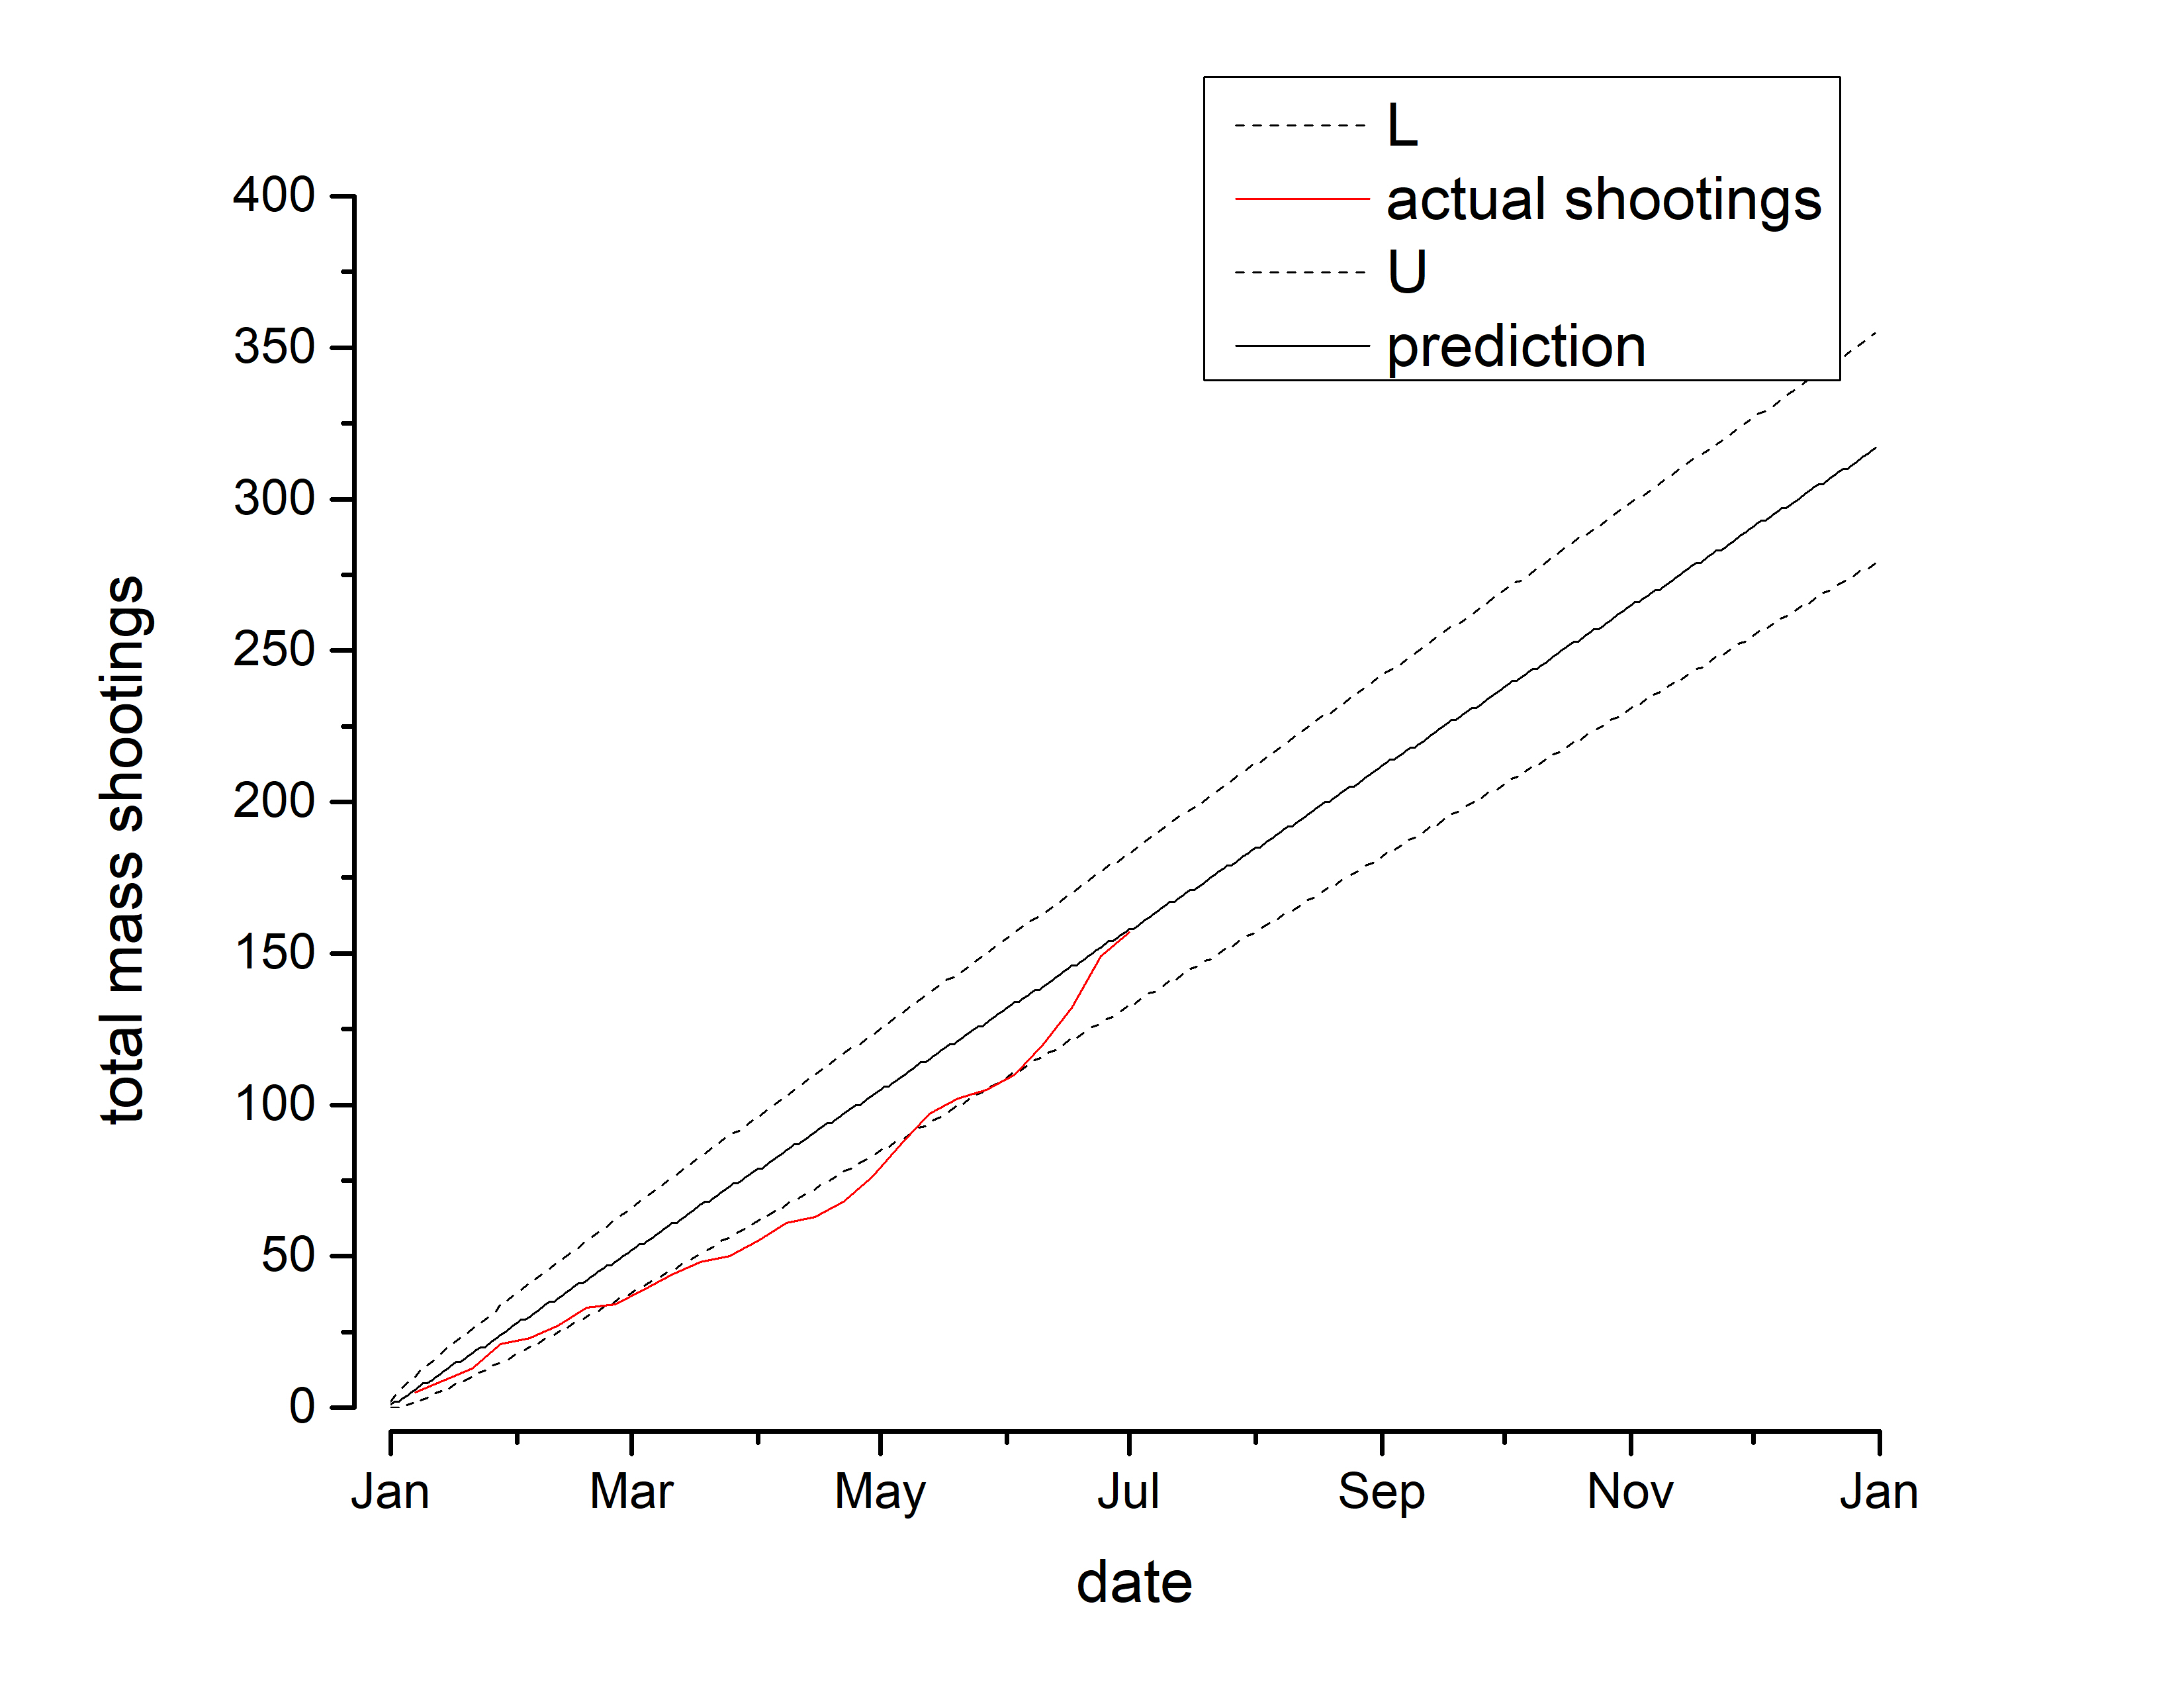
\includegraphics[scale=0.5]{Q9.jpg}
\caption{Data 2018 with the prediction intervals}
\end{figure}
Suppose we have two discrete random variables X,Y. Suppose X counts a certain event in a sample of total size n from a Poisson distribution with mean $\lambda$. Then X $\sim$ Poisson(n$\lambda$). Suppose Y is the future counts from the same Poisson distribution from a sample of total size m. Then Y $\sim$ Poisson(m$\lambda$). Let $\widehat{\lambda}$ = X/n, $\widehat{Y}$ = m$\widehat{\lambda}$ ($\widehat{Y}$=0.5m/n when X = 0)and $\widehat{var}$($\widehat{Y}$-Y) = m$\widehat{Y}$(1/n+1/m). Then ($\widehat{Y}$ - Y)/$\sqrt{\widehat{var}(\widehat{Y}-Y)}$ follows a standard normal distribution asymptotically.\par

To get the prediction interval [L,U] where L,U satisfy P$_{X,Y}$(L$\le$Y$\le$U)$\ge$1-2$\alpha$. Since ($\widehat{Y}$ - Y)/$\sqrt{\widehat{var}(\widehat{Y}-Y)}$ $\sim$ N(0,1), a 100(1-2$\alpha$)$\%$ two-sided confidence interval for Y is given by $\widehat{Y}$ $\pm$ z$_{1-\alpha}\sqrt{\widehat{var}(\widehat{Y}-Y)}$, where z$_{1-\alpha}$ is the value that P[Z$\le$z$_{1-\alpha}]$]=1-$\alpha$, Z$\sim$N(0,1). Since we are only considering integer values of Y, we can see that [L,U] is given by \par [$\lfloor$$\widehat{Y}$- z$_{1-\alpha}\sqrt{\widehat{var}(\widehat{Y}-Y)}$$\rfloor$,$\lceil$$\widehat{Y}$+z$_{1-\alpha}\sqrt{\widehat{var}(\widehat{Y}-Y)}$$\rceil$].
\section{Conclusion}
After all these tests, our group finally got a conclusion.
\par The occurrence of mass shootings in the United States depends on weekdays, and it is more likely to happen in weekends. This makes sense, since in weekends people have more free time, and the shooter may have more time to prepare the assault. Since it depends on weekdays, we cannot analyze the daily data. After analyzing the weekly data, we found the numbers of occurrence of mass shooting in one week may follow a Poisson distribution in a short period, like a single year, but not in a long period.
\par And the reason may be that the occurrence of mass shooting is not a random event. People may tend to shoot when the social security is not so good, it depends on many social factors, so in a short period, when the social and national conditions don't change a lot, the the numbers of occurrence of mass shooting in one week may follow a Poisson distribution, but in a long period, since the society and country are changing, which may cause the parameter $k$ of the Poisson distribution to change, that means at different years, the numbers of occurrence of mass shooting in one week may follow Poisson distributions with different parameter $k$,so we can't simply use Poisson distribution to test the data in a long period.
\par Our conclusion is helpful to prevent mass shooting. Because the different parameter $k$ at different years in some way may reflect the social security at that year, lower $k$ reflects better social security, while higher $k$ reflects the president should try to strengthen the social security. Also, the higher probability of mass shooting happening in weekends may give the government some hints to prevent mass shootings.
\section{Reference}
\begin{enumerate}[-]
\item Gun Violence Archive. Mass shootings. \url{http://www.shootingtracker.com/}
\item K. Krishnamoorthy and Jie Peng. Improved closed-form prediction intervals for binomial and poisson
distributions. Journal of Statistical Planning and Inference, 141(5):1709 – 1718, 2011.
\item VV Patil and HV Kulkarni. Comparison of confidence intervals for the poisson mean: some new aspects.
REVSTAT–Statistical Journal, 10(2):211–227, 2012.
\item D. Spiegelhalter and A. Barnett. London murders: a predictable pattern? Significance, 6(1):5–8,
2009. \url{onlinelibrary.wiley.com/doi/10.1111/j.1740-9713.2009.00334.x/abstract} [Online;
accessed 5-July-2015]
\end{enumerate}
\section{Appendix}
\begin{enumerate}[-]
\item Mathematica code for Ex2
\begin{figure}[H]
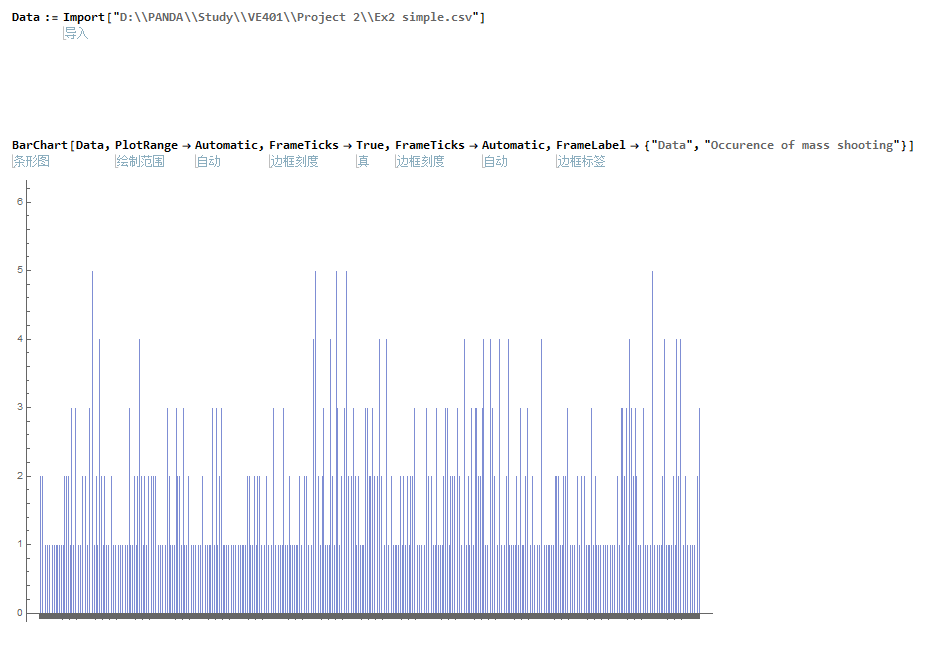
\includegraphics[scale=0.5]{MQ2.jpg}
\end{figure}
\newpage
\item Mathematica code for Ex4
\begin{figure}[H]
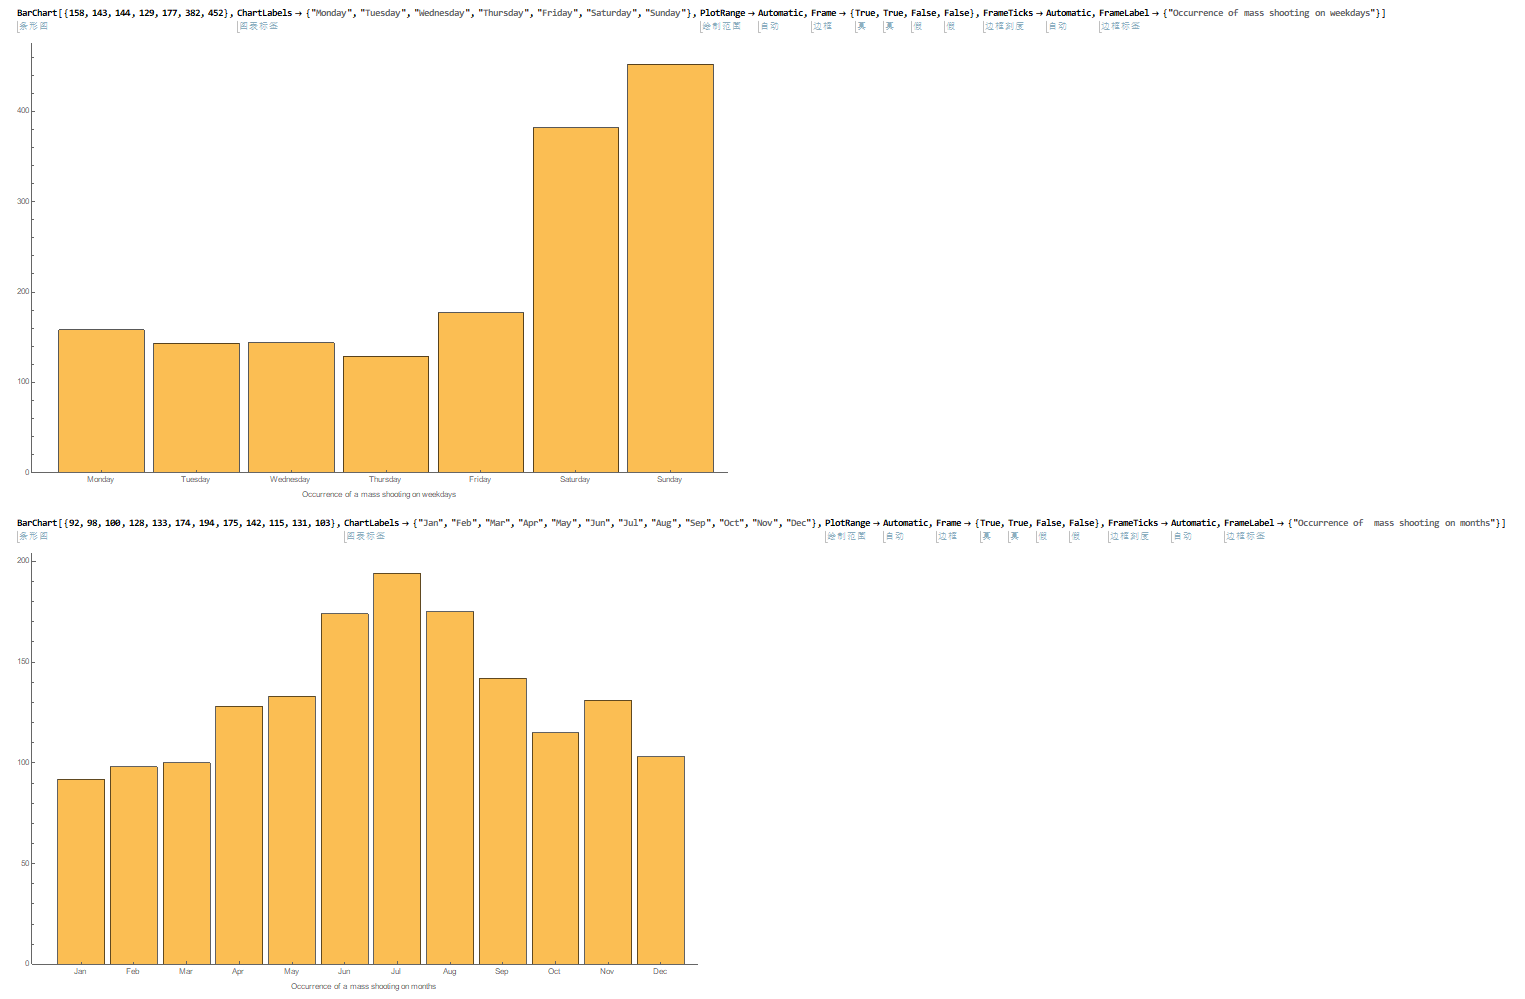
\includegraphics[scale=0.35]{MQ4.jpg}
\end{figure}
\newpage
\item Mathematica code for Ex7 and Ex8
\begin{figure}[H]
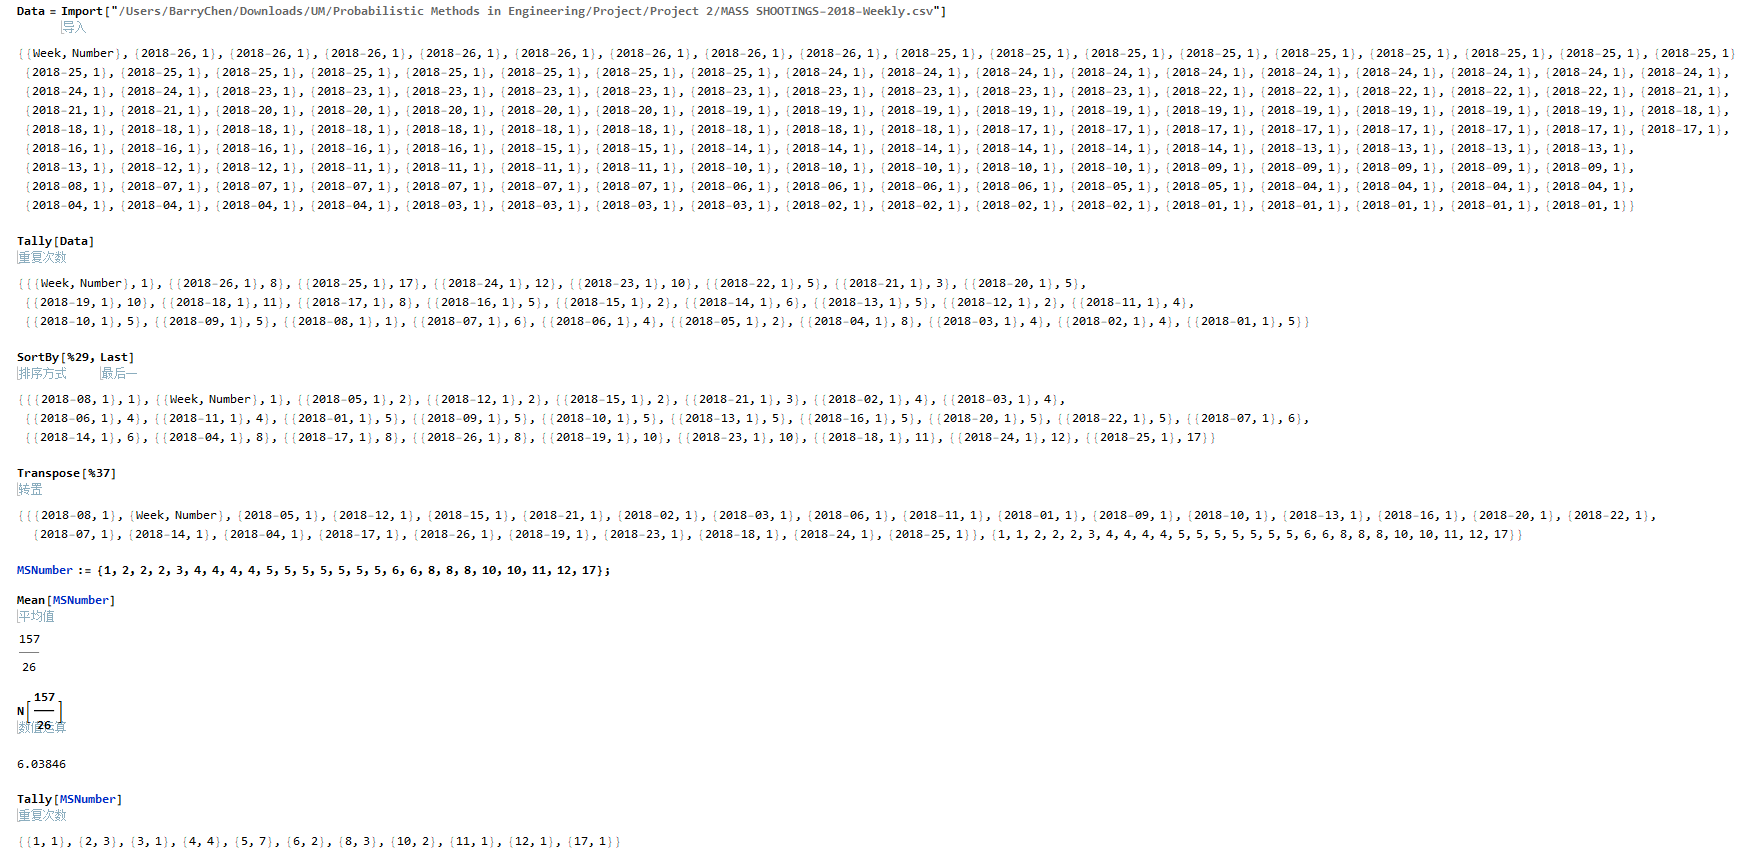
\includegraphics[scale=0.3]{MQ7-1.jpg}
\end{figure}
\begin{figure}[H]
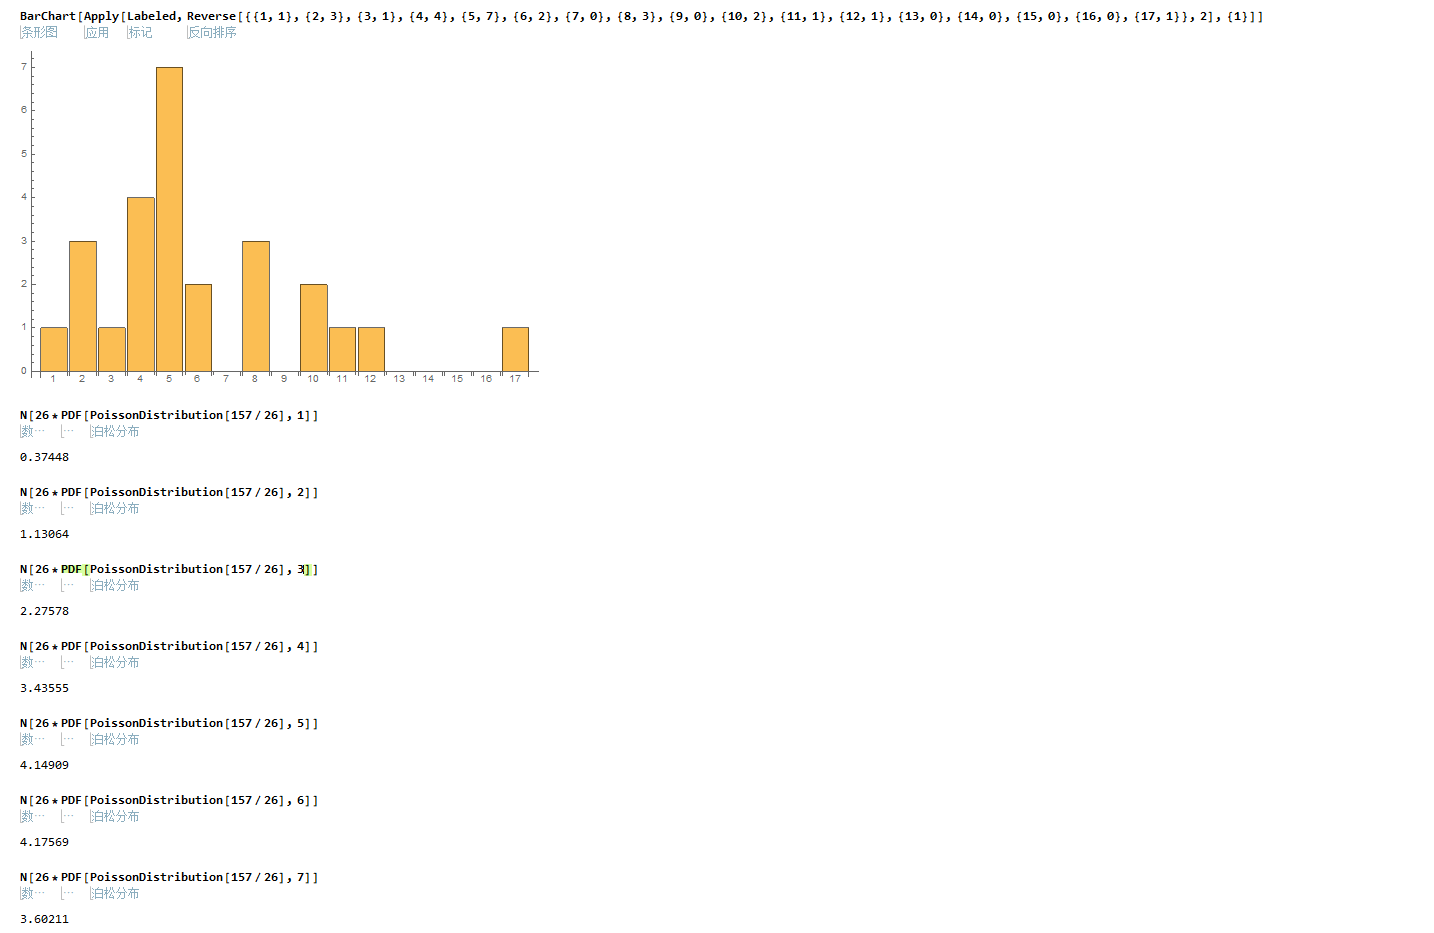
\includegraphics[scale=0.3]{MQ7-2.jpg}
\end{figure}
\begin{figure}[H]
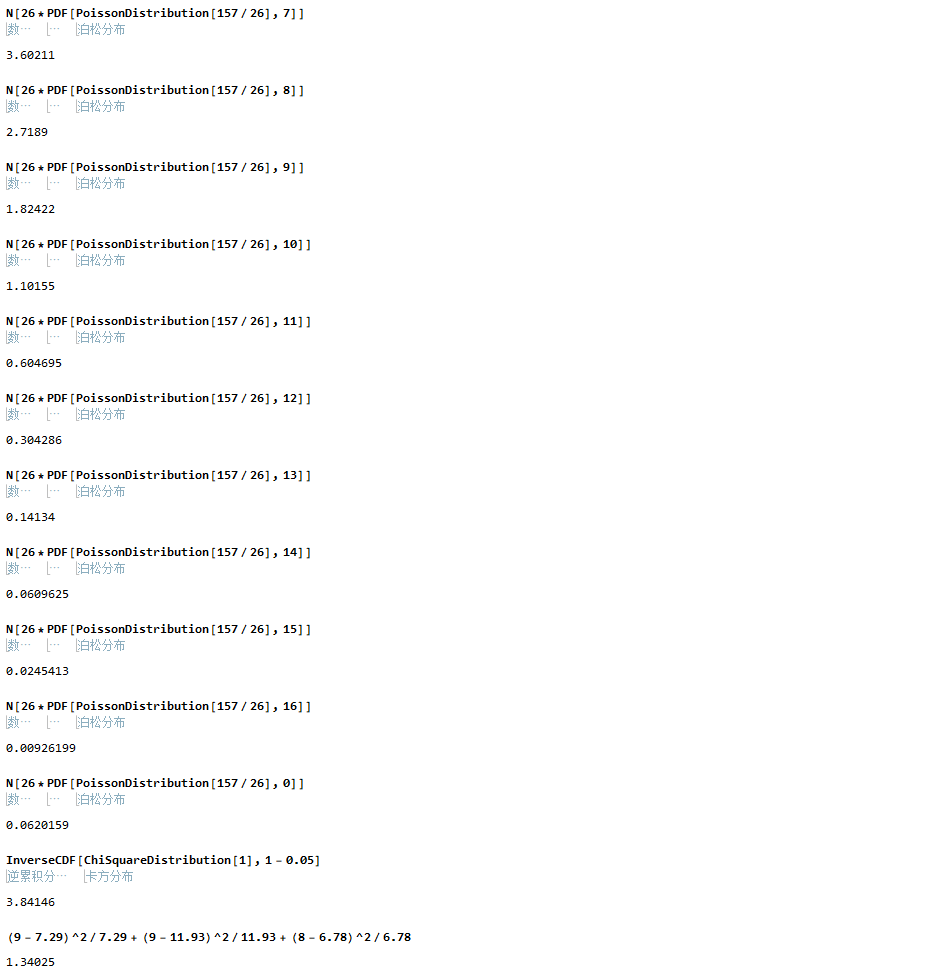
\includegraphics[scale=0.3]{MQ7-3.jpg}
\end{figure}
\end{enumerate}
\end{document}
